\chapter{System design}
\label{chap:design}

\section{Model building}
Model development and model deployment are separate stages. The
notebook uses labelled synthetic activity for training and
evaluation. The deployed local scorer accepts unlabeled activity,
loads an already-created bundle, and produces a ranked report. The
dashboard does not retrain estimators when an analyst submits a folder.

\subsection{Implementation code}
Notebook cells implement data inspection, aggregation, label
construction, group splitting, model fitting, validation selection,
test evaluation, visualisation, and bundle persistence. The scoring
core shares the feature-generation contract used by the application.
The selected feature list is included in the bundle so the inference
path can insert missing columns and order inputs consistently.

\subsection{Model planning and training/testing split}
The notebook applies an outer \code{StratifiedGroupKFold} splitter with
five folds and a fixed seed to hold out test users. An inner
four-fold stratified group split with a separate seed partitions the
remaining users into training and validation groups. The first
split produced by each configured splitter is used. The identifier
groups are checked for overlap. If any partition lacks a positive
employee-day, the notebook stops rather than reporting an unusable
comparison.

The saved evaluation partition contains 66,118 employee-days and 289
positive rows. The group split is a stronger safeguard against
same-user leakage than a random row split, though it does not solve
temporal drift, release-to-release shift, or differences between
synthetic and real activity.

\subsection{Training}
The supervised estimators are fitted on training labels only.
Isolation Forest is fitted on training features and does not use the
incident labels. The Random Forest augmentation routine creates one
count-perturbed positive example per positive training row. It samples
positive anchors, applies a log-normal multiplier, resamples event
counts from Poisson distributions, and reconstructs after-hours,
device-connection, and attachment counts while preserving
source-level relationships. Validation Average Precision decides
whether the augmented version is retained. Test data is not used for
that decision.

\subsection{Testing}
The notebook evaluates the selected estimators on the held-out test
partition. It chooses the queue rate on validation data by searching a
set of candidate capacities and maximising validation F1. The saved
rate is one percent. At that rate the test set contributes 662
employee-days to the queue. A five-percent capacity is also retained
as a comparison reference. These are ranking capacities, not fixed
probability thresholds.

\section{System architecture}
\begin{figure}[H]
\centering
\begin{tikzpicture}[
  node distance=9mm and 10mm,
  unit/.style={draw,rounded corners,align=center,text width=0.38\textwidth,minimum height=12mm},
  arrow/.style={-{Stealth[length=2mm]},thick}
]
\node[unit] (browser) {React dashboard\\folder selection, progress, queue, details};
\node[unit,right=of browser] (api) {FastAPI service\\health, progress, analysis, employee detail};
\node[unit,below=of api] (core) {Forensic core\\chunked parsing, features, model scoring};
\node[unit,left=of core] (files) {Local inputs and artifacts\\five CSVs, model bundle, report outputs};
\draw[arrow] (browser)--node[above]{HTTP / JSON and upload}(api);
\draw[arrow] (api)--(core);
\draw[arrow] (files)--(core);
\draw[arrow] (core)--(api);
\draw[arrow] (api)--(browser);
\end{tikzpicture}
\caption{Application component architecture}
\label{fig:architecture}
\end{figure}

\subsection{Component responsibilities}
\textbf{React client.} The client checks health, collects files using a
directory input, uploads the selected CSVs, polls progress, and
renders the report. It supports employee search and status filtering,
and requests activity detail for a selected employee.

\textbf{FastAPI service.} The service validates uploaded filenames,
stages accepted files in a temporary directory, invokes the scoring
core, stores the most recent in-memory results for detail requests,
and writes CSV exports. It exposes health and progress endpoints for
the UI. A lock serialises analysis requests in this single-process
prototype.

\textbf{Forensic core.} The core checks model availability and required
input files, parses the logs in chunks, builds user-day features,
orders model inputs, scores with each estimator, calculates consensus
ranks, generates reasons, and formats selected activity rows.

\textbf{Model bundle.} The bundle contains the four fitted models and
the feature-column list. It is loaded with joblib. Bundle files are
trusted local artifacts; loading joblib from an untrusted source is
not safe and must not be permitted in an operational deployment.

\section{Use-case model}
\begin{figure}[H]
\centering
\begin{tikzpicture}[
  usecase/.style={draw,ellipse,align=center,text width=0.31\textwidth,minimum height=10mm},
  actor/.style={draw,rounded corners,align=center,text width=0.17\textwidth,minimum height=9mm},
  arrow/.style={-{Stealth[length=2mm]},thick}
]
\node[actor] (analyst) {Analyst};
\node[usecase,right=23mm of analyst,yshift=22mm] (select) {Select five activity logs};
\node[usecase,below=of select] (run) {Run local analysis};
\node[usecase,below=of run] (queue) {Review prioritised employees};
\node[usecase,below=of queue] (detail) {Inspect employee-day aggregates};
\node[usecase,below=of detail] (export) {Save report outputs};
\draw[arrow] (analyst)--(select);
\draw[arrow] (analyst)--(run);
\draw[arrow] (analyst)--(queue);
\draw[arrow] (analyst)--(detail);
\draw[arrow] (analyst)--(export);
\end{tikzpicture}
\caption{Primary analyst use cases}
\label{fig:use-case}
\end{figure}

The analyst is the principal interactive actor. Data custodians and
model maintainers are operational stakeholders but are not
authenticated application roles. The use-case diagram intentionally
does not model automated decision-making: the application ranks
records and exposes information for a human process outside the
prototype.

\section{Activity diagram}
\begin{figure}[H]
\centering
\begin{tikzpicture}[
  node distance=7mm,
  process/.style={draw,rounded corners,align=center,text width=0.65\textwidth,minimum height=8mm},
  decision/.style={draw,diamond,aspect=3,align=center,text width=0.32\textwidth,inner sep=1pt},
  arrow/.style={-{Stealth[length=2mm]},thick}
]
\node[process] (start) {Start local UI and check API/model health};
\node[process,below=of start] (choose) {Choose folder and collect activity files};
\node[decision,below=of choose] (complete) {All five required logs present?};
\node[process,below left=of complete] (error) {Display missing-file message; allow correction};
\node[process,below right=of complete] (upload) {Upload, stage temporarily, aggregate, score};
\node[process,below=18mm of upload] (show) {Show queue, summary, model ranks, and selected activity};
\node[process,below=of show] (end) {Analyst verifies original evidence and records outcome externally};
\draw[arrow] (start)--(choose);
\draw[arrow] (choose)--(complete);
\draw[arrow] (complete)--node[above left]{No}(error);
\draw[arrow] (complete)--node[above right]{Yes}(upload);
\draw[arrow] (upload)--(show);
\draw[arrow] (show)--(end);
\end{tikzpicture}
\caption{Analysis and review activity}
\label{fig:activity}
\end{figure}

\section{Sequence diagram}
\begin{figure}[H]
\centering
\begin{tikzpicture}[
  actor/.style={draw,rounded corners,align=center,text width=0.18\textwidth,minimum height=8mm},
  arrow/.style={-{Stealth[length=2mm]},thick},
  node distance=10mm and 11mm
]
\node[actor] (ui) {React UI};
\node[actor,right=of ui] (api) {FastAPI};
\node[actor,right=of api] (core) {Scoring core};
\node[actor,right=of core] (bundle) {Model bundle};
\draw[dashed] (ui.south)--++(0,-9.5);
\draw[dashed] (api.south)--++(0,-9.5);
\draw[dashed] (core.south)--++(0,-9.5);
\draw[dashed] (bundle.south)--++(0,-9.5);
\draw[arrow] ([yshift=-10mm]ui.south)--node[above]{Upload selected files}([yshift=-10mm]api.south);
\draw[arrow] ([yshift=-23mm]api.south)--node[above]{Validate and stage files}([yshift=-23mm]core.south);
\draw[arrow] ([yshift=-36mm]core.south)--node[above]{Load fitted estimators}([yshift=-36mm]bundle.south);
\draw[arrow] ([yshift=-49mm]bundle.south)--node[below]{Models and feature schema}([yshift=-49mm]core.south);
\draw[arrow] ([yshift=-62mm]core.south)--node[above]{Ranked data and activity detail}([yshift=-62mm]api.south);
\draw[arrow] ([yshift=-75mm]api.south)--node[below]{JSON report and progress}([yshift=-75mm]ui.south);
\end{tikzpicture}
\caption{High-level sequence for a folder analysis}
\label{fig:sequence}
\end{figure}

\section{Data design}
The project uses file-based input and output rather than a relational
database. The main logical records are source events, employee-day
aggregates, model scores, employee summaries, and optional display
names. A user-day key joins the source aggregates. The user key joins
day rows to an employee summary.

\begin{table}[H]
\centering
\tablefont
\caption{Logical data entities}
\label{tab:entities}
\begin{tabularx}{\textwidth}{|p{0.23\textwidth}|p{0.30\textwidth}|Y|}
\hline
\textbf{Entity} & \textbf{Key fields} & \textbf{Purpose}\\\hline
Source event & user, timestamp, source-specific fields & Original observed event; retained in input files.\\\hline
Employee-day row & user, day, feature columns & Aggregated evidence used by the estimators.\\\hline
Model score row & user, day, four model ranks, consensus & Relative model ranking for one employee-day.\\\hline
Employee summary & user, active days, maxima, agreement, status & Review queue record and explanatory summary.\\\hline
Name lookup & user, name & Optional display-only lookup; not used as model input.\\\hline
\end{tabularx}
\end{table}

The service stores the last successful analysis in process memory for
employee-detail requests. The in-memory state is not durable, is
shared only within the running process, and is replaced by the next
analysis. The CSV exports are convenient report artifacts but do not
include a transactional case history. A production design should
define stable identifiers, access permissions, retention periods,
integrity checks, backup policy, and an append-only audit trail.

\section{API design}
\begin{table}[H]
\centering
\tablefont
\caption{Local API endpoints}
\label{tab:api}
\begin{tabularx}{\textwidth}{|p{0.19\textwidth}|p{0.28\textwidth}|p{0.42\textwidth}|}
\hline
\textbf{Method and route} & \textbf{Purpose} & \textbf{Result and error behaviour}\\\hline
\code{GET /api/health} & Report model-bundle readiness. & Returns a readiness Boolean and explanatory message.\\\hline
\code{GET /api/progress} & Read current analysis stage. & Returns percentage, stage text, and active state.\\\hline
\code{POST /api/analyze} & Analyse an existing local folder path. & Returns employee records and summary; invalid folders or scoring failures return errors.\\\hline
\code{POST /api/analyze-upload} & Receive selected activity files. & Validates required names, rejects duplicates, stages files temporarily, and returns ranked results.\\\hline
\code{POST /api/employee} & Request detail for one user. & Returns model scores and selected daily activity; returns conflict before analysis or not-found for unknown users.\\\hline
\end{tabularx}
\end{table}

The browser uses the upload route so the backend can operate on a
temporary staged folder. File names are reduced to their basename and
compared with an allowlist of required and optional names. This is a
useful input constraint, but it is not a complete security boundary:
the application has no user authentication, rate limiting, CSRF
protection, or production-grade isolation. It is documented to run on
the loopback interface and should not be exposed to an untrusted
network.

\section{UI design}
The React interface uses a dark sidebar, a light review workspace, a
folder-selection card, an expandable model guide, and an analysis
progress panel. After scoring, the dashboard presents summary counts,
flagged employees, a searchable directory, and employee activity
details. Status language is deliberately framed as review priority.

\begin{figure}[H]
\centering
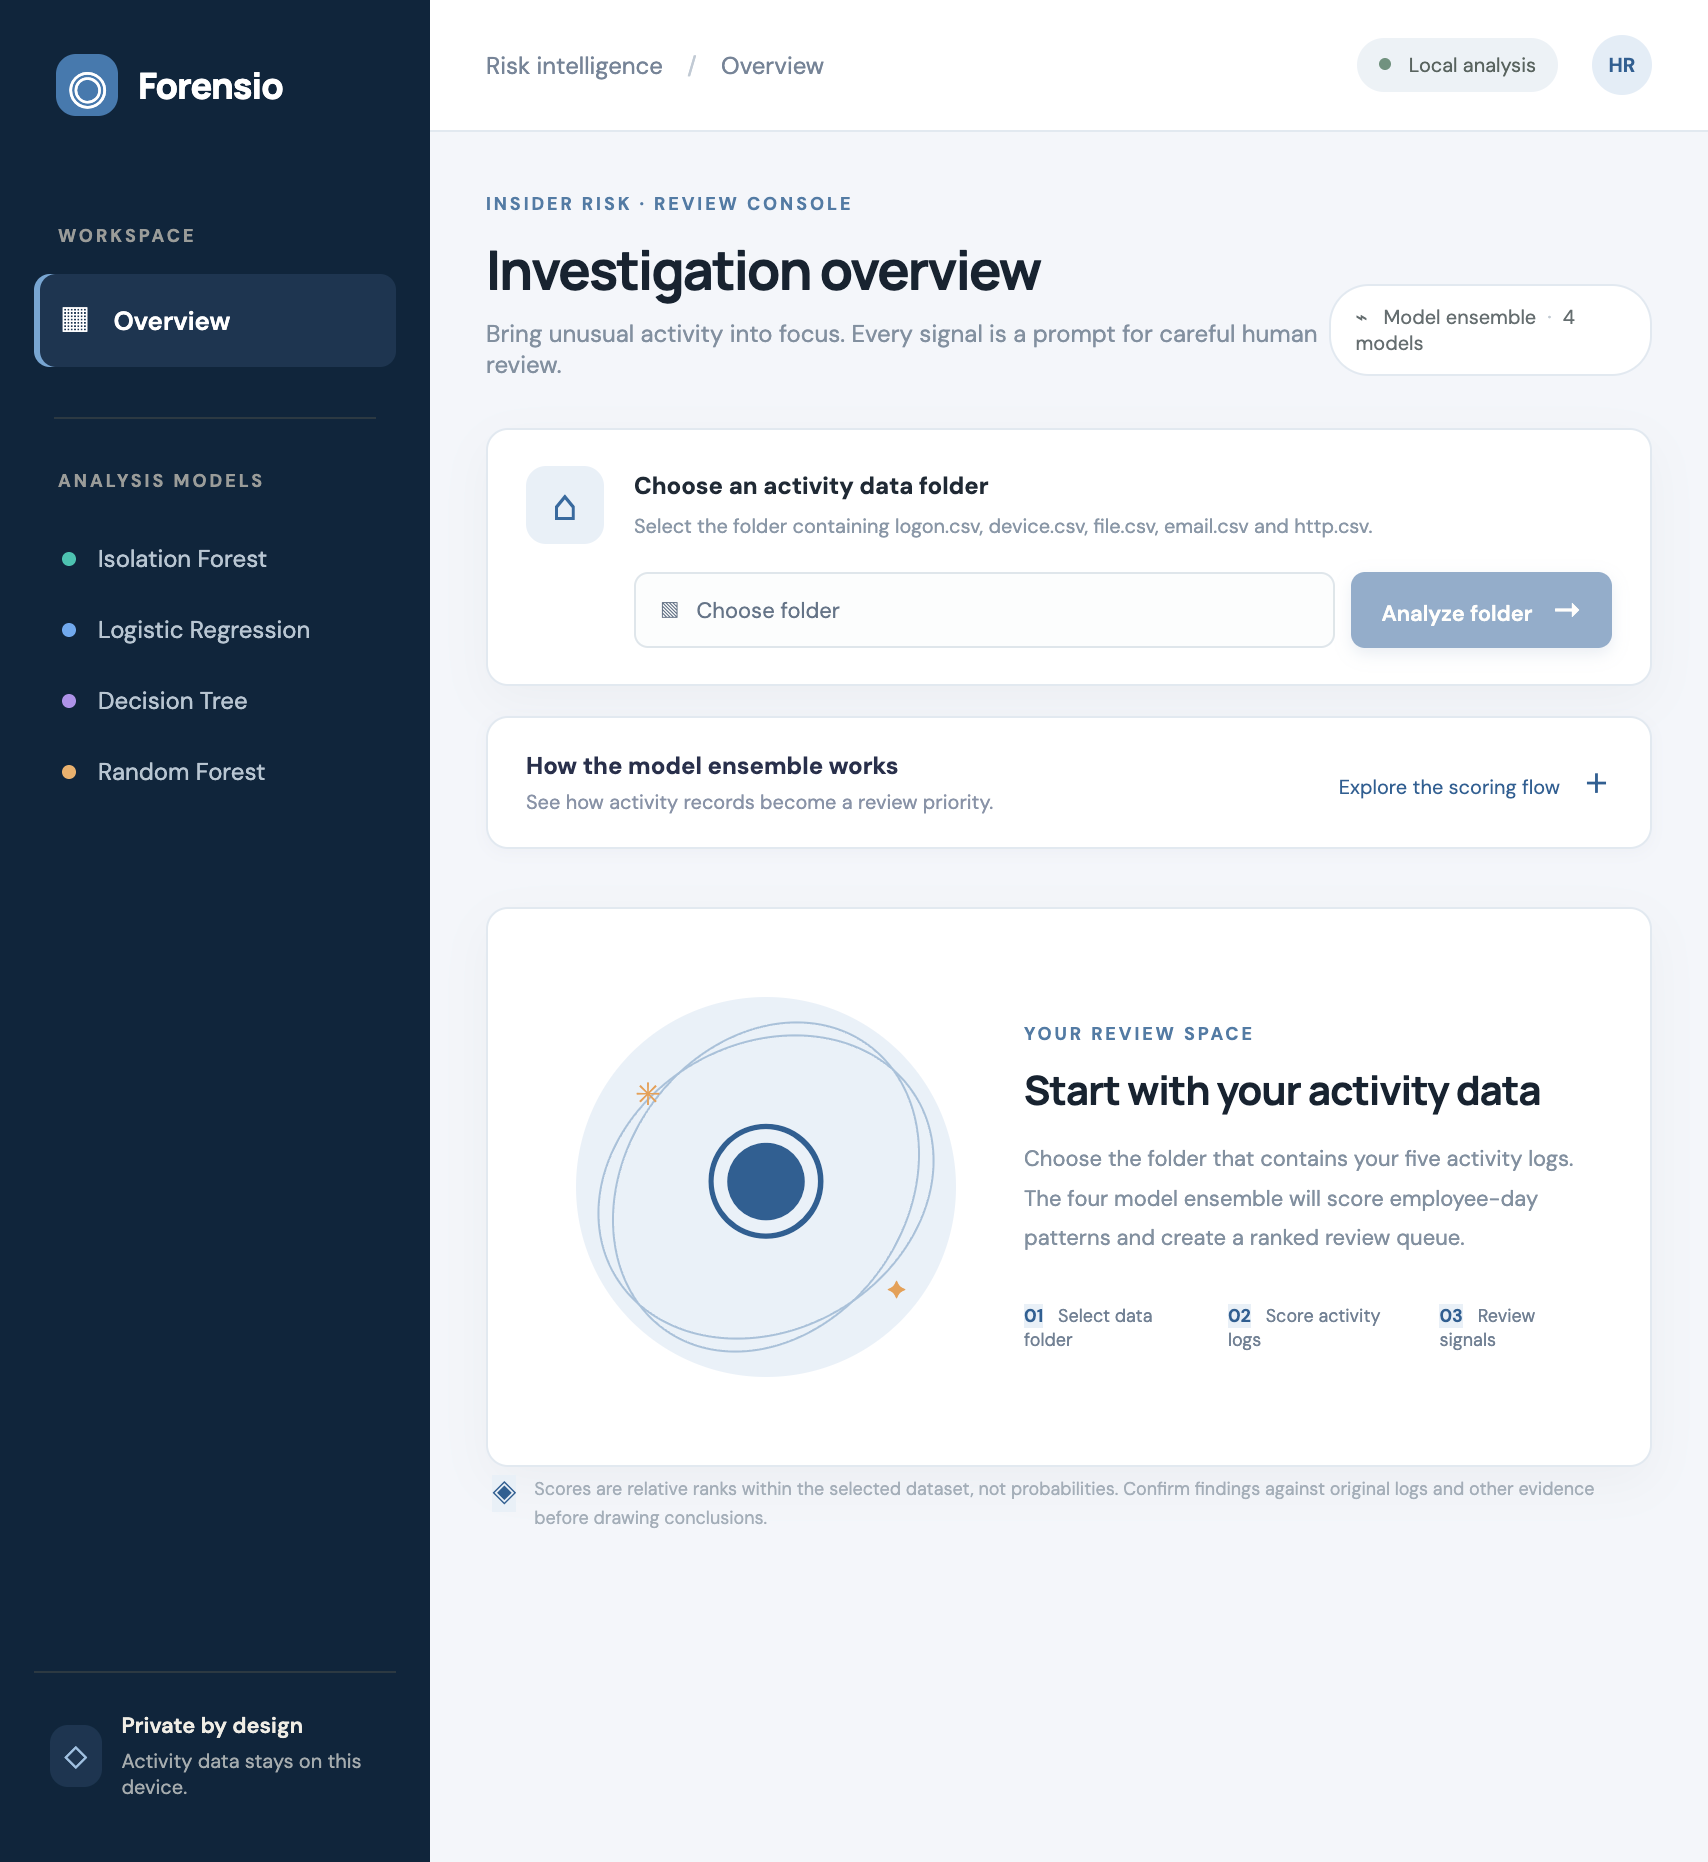
\includegraphics[width=0.78\textwidth,height=0.65\textheight,keepaspectratio]{ui_react_landing.png}
\caption{Forensio React dashboard landing state}
\label{fig:ui-landing}
\end{figure}

\begin{figure}[H]
\centering
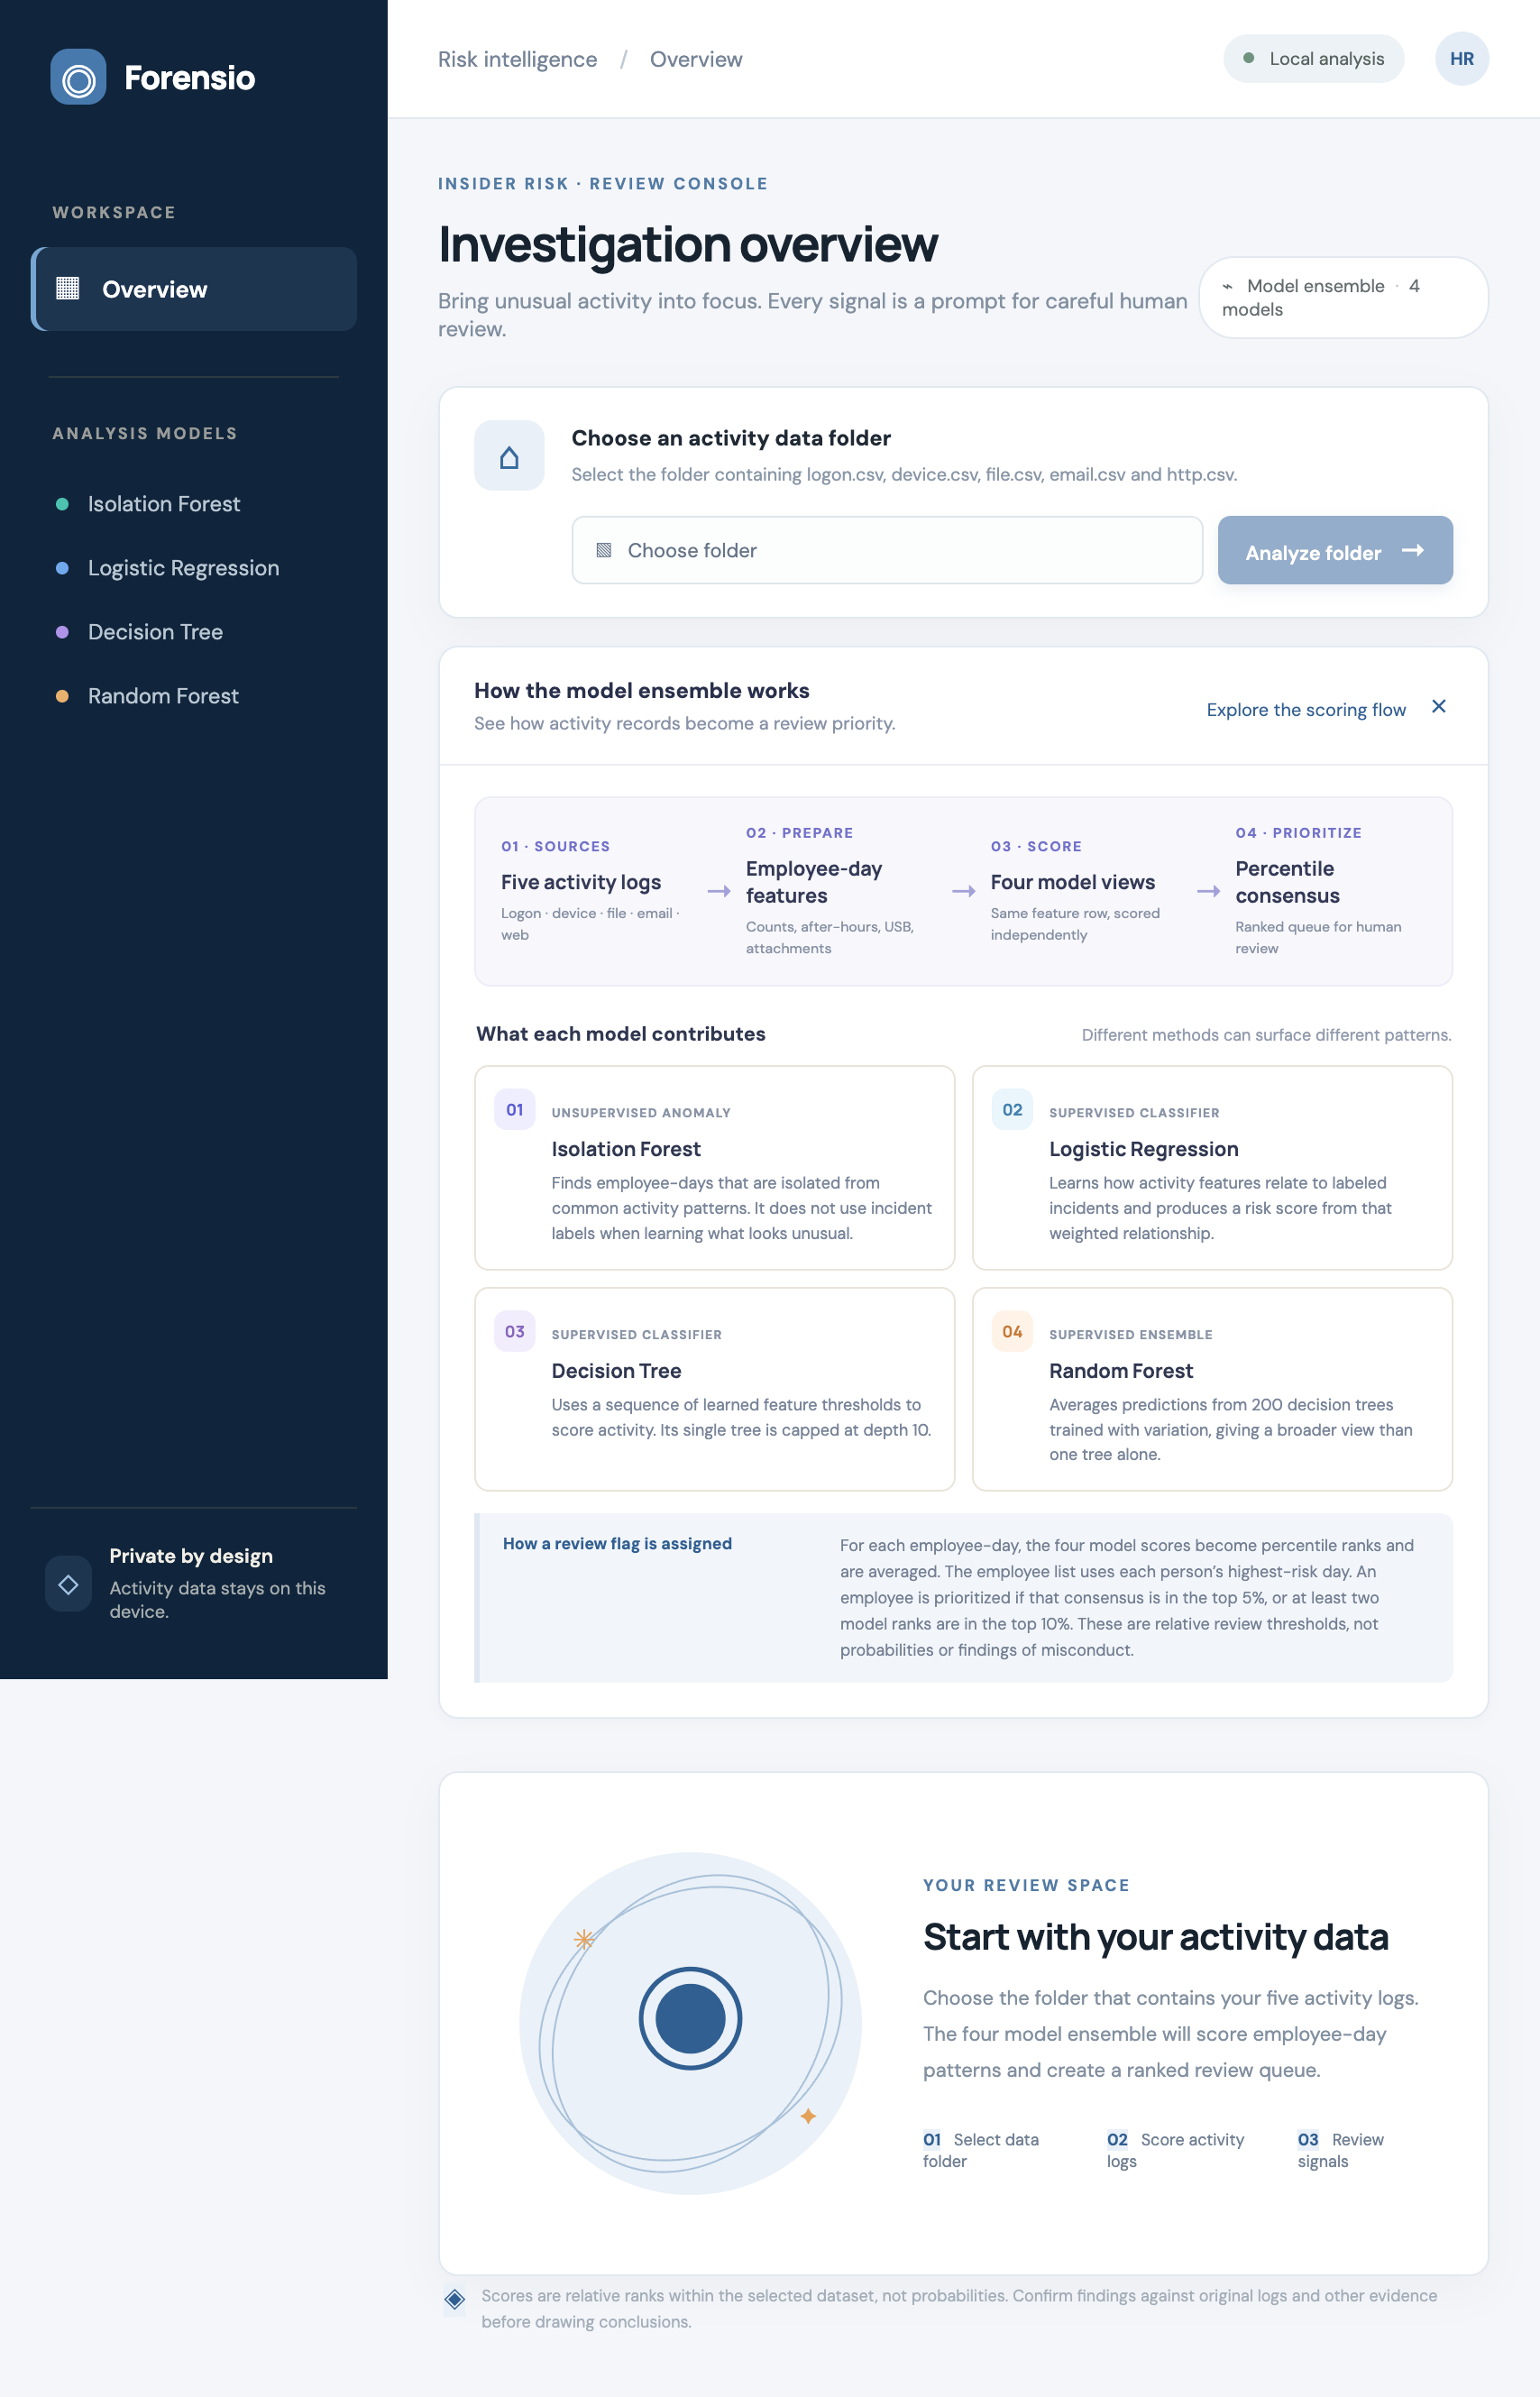
\includegraphics[width=0.69\textwidth,height=0.72\textheight,keepaspectratio]{ui_react_model_guide.png}
\caption{Expanded model guide and scoring explanation}
\label{fig:ui-guide}
\end{figure}

The landing screenshot illustrates the initial local-analysis state.
The model-guide screenshot describes the four methods and the
percentile-based dashboard rule. Captures are snapshots of the
interface and may not show every interaction state or the latest visual
change. The report does not treat a screenshot as proof that every
workflow has been tested end to end.

\subsection{Interaction states}
\begin{table}[H]
\centering
\tablefont
\caption{User-interface states and visible response}
\label{tab:ui-states}
\begin{tabularx}{\textwidth}{|p{0.21\textwidth}|p{0.37\textwidth}|Y|}
\hline
\textbf{State} & \textbf{Trigger} & \textbf{Expected interface response}\\\hline
Checking service & Page load or API not reachable. & Show availability message and retry the health request.\\\hline
Ready & Model bundle is present and API is reachable. & Enable folder selection and analysis when required inputs are found.\\\hline
Incomplete folder & One or more required CSVs are absent. & List the missing filenames and disable analysis.\\\hline
Uploading & Browser sends selected files. & Display upload progress and disable repeated submission.\\\hline
Scoring & API aggregates and scores records. & Poll progress and show current stage and estimated remaining time.\\\hline
Successful analysis & API returns a report. & Render summary, flagged queue, searchable directory, and details.\\\hline
Failed analysis & Service or parser returns an error. & Show an error message so the operator can correct input or inspect service logs.\\\hline
\end{tabularx}
\end{table}

\subsection{Accessibility and usability}
The React implementation uses native form controls, descriptive labels
for the directory picker, a live status region for analysis progress,
and a progress bar with current and maximum values. Search and status
filters reduce navigation effort when the employee list is large. A
textual model guide explains the distinction between model families
and the review rule.

Further accessibility work should include keyboard-only workflow
testing, focus management after analysis, screen-reader testing of
dynamic results, high-contrast verification, and clear focus
indicators. The current screenshots are visual evidence of layout,
not a formal accessibility conformance assessment.

\chapter{Results and discussion}
\label{chap:results}

\section{Testing approach}
The repository contains saved data-quality and evaluation artifacts,
but no dedicated automated test suite was identified. This report
therefore distinguishes checks reflected in the source and saved
outputs from tests that would still need to be run. The test cases in
Appendix 10.4 are a verification plan unless an execution result is
explicitly recorded. They must not be interpreted as all passing.

The strongest available quantitative evidence is the saved
employee-day model comparison and confusion-count output. The saved
training notebook fixes random seeds for splitting and estimators;
however, reproducibility also depends on package versions, data-file
integrity, notebook execution order, and model artifact provenance.

\section{Model planning and evaluation protocol}
The labelled table contains 330,452 employee-days and 1,364 positives.
The held-out test partition has 66,118 employee-days, including 289
positives. The selected queue size is 662 rows at one percent. The
one-percent capacity was selected on validation data only by F1 search;
the estimator variant was selected on validation Average Precision.
The test split was reserved for reporting.

Evaluation is made at the employee-day level. The test confusion
matrix describes whether a row is inside a known incident interval
under the answer-file label rule. It does not state whether a person
committed misconduct, nor does it establish the correctness of an
investigative outcome.

\section{Validation design and class imbalance}
The saved employee-day table is strongly imbalanced: 1,364 of 330,452
rows are positive under the incident-window rule. A model can therefore
rank a large number of ordinary-looking records above the rare positive
class without a large change in overall accuracy. This affects both
training and evaluation. Class weighting changes the penalty associated
with misclassified examples during supervised fitting, but it does not
create new independent incidents. Synthetic augmentation adds derived
training examples according to a transformation rule; it must not be
counted as additional observed evidence.

The project uses user-group separation so that records from one
synthetic person are not split across training, validation, and test.
This addresses a specific leakage risk: daily rows from one user may
share activity levels or stable habits. If some rows from the same user
were present in training while other rows were held out, a model might
benefit from person-specific regularities that would not be available
for a new user. Group separation makes the test more informative about
unseen users, although it does not answer whether the model will
transfer to a different organisation, time period, or activity system.

Model selection and evaluation are separated by purpose. Training data
fit model parameters. Validation data compare the baseline and
augmented Random Forest candidates and select the queue capacity by
F1. Test data are held aside for reporting. Using test results to
change a feature, a model parameter, or the queue rate would convert
the test set into additional validation data and make the reported
performance optimistic. If the model is revised after this report, a
new test partition or a prospective evaluation is needed for an
unbiased estimate.

The single saved split also has sampling uncertainty. With only 289
positive test rows, a change of several correctly ranked records can
materially change precision and recall. This report presents the saved
point estimates and confusion counts, but not confidence intervals or
repeated group-split variability. A stronger study would use repeated
stratified group splits or a time-based holdout, report the distribution
of rare-class metrics, and explain how the split design matches the
intended deployment question. The test design should be documented
before examining performance, rather than selected after seeing which
partition produces a favourable score.

A time-based holdout answers a different question from a random
user-group holdout. Grouped partitions ask whether the model ranks
records from users it did not train on. Time-based partitions ask
whether a model trained on earlier activity remains useful on later
activity. Both questions can matter. A chronological design may expose
changes in work patterns, software systems, or event collection that a
random partition does not reveal. The current results should therefore
be described as one grouped holdout experiment, not as evidence of
long-term stability.

\section{Comparison of models}
\begin{table}[H]
\centering
\tablefont
\caption{Saved model comparison at the validation-selected one-percent queue capacity}
\label{tab:model-results}
\begin{tabularx}{\textwidth}{|p{0.18\textwidth}|R|R|R|R|R|}
\hline
\textbf{Model} & \textbf{Val. AP} & \textbf{Test P@1\%} & \textbf{Test R@1\%} & \textbf{Test F1} & \textbf{Test AP}\\\hline
Random Forest & 0.275 & 0.144 & 0.329 & 0.200 & 0.158\\\hline
Decision Tree & 0.185 & 0.121 & 0.277 & 0.168 & 0.104\\\hline
Logistic Regression & 0.027 & 0.003 & 0.007 & 0.004 & 0.027\\\hline
Isolation Forest & 0.016 & 0.027 & 0.062 & 0.038 & 0.027\\\hline
\end{tabularx}
\end{table}

At the saved one-percent capacity, Random Forest has the highest test
Average Precision among the four listed models and the highest test
precision, recall, and F1 at that fixed capacity. This is an
observation about the saved partition and configuration only. The
Decision Tree also ranks some known positive days, while Logistic
Regression and Isolation Forest perform less strongly at the
one-percent operating point. The results do not establish that a
Random Forest is universally preferable for insider-risk work.

\begin{table}[H]
\centering
\tablefont
\caption{Random Forest confusion matrix at the one-percent test queue}
\label{tab:rf-confusion}
\begin{tabularx}{0.8\textwidth}{|p{0.29\textwidth}|R|R|}
\hline
 & \textbf{Predicted not queued} & \textbf{Predicted queued}\\\hline
\textbf{Actual negative label} & 65,262 & 567\\\hline
\textbf{Actual positive label} & 194 & 95\\\hline
\end{tabularx}
\end{table}

The one-percent queue contains 95 known positive employee-days and 567
rows that do not match a known positive label. It misses 194 of the
289 positive rows. These false-positive and false-negative terms are
defined relative to the synthetic incident-window label, not to
confirmed real-world outcomes. A row labelled negative may still
require attention for reasons outside the benchmark's labels.

\begin{table}[H]
\centering
\tablefont
\caption{Random Forest comparison at a five-percent capacity reference}
\label{tab:five-percent}
\begin{tabularx}{\textwidth}{|p{0.30\textwidth}|R|R|R|}
\hline
\textbf{Metric} & \textbf{One percent} & \textbf{Five percent} & \textbf{Interpretation}\\\hline
Queue size & 662 & 3,306 & Number of test employee-days selected.\\\hline
Known positives retrieved & 95 & 178 & Test positive labels inside the queue.\\\hline
Precision & 0.144 & 0.054 & Positive labels per selected record.\\\hline
Recall & 0.329 & 0.616 & Positive labels found out of 289.\\\hline
F1 & 0.200 & 0.099 & Harmonic mean of precision and recall at each capacity.\\\hline
\end{tabularx}
\end{table}

Increasing the capacity from one to five percent retrieves more known
positive days but also adds more records to the analyst queue. The
one-percent setting has higher precision and F1 in the saved test
result, while five percent has higher recall. This trade-off is
expected in a ranked review process and should be selected according to
real operational capacity and the consequences of missed leads.

\section{Evaluation metrics}
Let \(P\) be the set of test employee-days labelled positive and
\(Q_k\) the \(k\) highest-scored rows. At a fixed queue size:
\[
\operatorname{Precision@}k = \frac{|Q_k\cap P|}{k},
\qquad
\operatorname{Recall@}k = \frac{|Q_k\cap P|}{|P|}.
\]
Precision measures the positive-label fraction among selected rows.
Recall measures the positive-label fraction retrieved. F1 is the
harmonic mean of precision and recall. Average Precision summarizes
ranking quality over score thresholds and does not depend on a single
fixed queue cutoff.

Accuracy is the fraction of all records correctly classified at a
chosen threshold. With 289 positive rows among 66,118 test rows, a
model that predicts almost everything negative can attain high
accuracy while retrieving few positives. Accuracy must therefore be
read alongside positive-class metrics and queue size.

\section{Capacity selection and operational interpretation}
A review queue is a resource allocation mechanism. If the capacity is
\(k\) rows, the selected set contains the highest-ranked \(k\) records.
For a positive set \(P\), precision and recall are
\[
 \operatorname{Precision@}k=\frac{|Q_k\cap P|}{k},
 \qquad
 \operatorname{Recall@}k=\frac{|Q_k\cap P|}{|P|}.
\]
This makes the workload explicit: a one-percent employee-day queue
selects about one percent of records, whereas a five-percent queue
requires five times as many employee-day reviews. The unit matters; a
percentage of days is not a percentage of employees or cases.

The validation F1 search chooses a point that balances precision and
recall under the benchmark labels. It does not encode the actual cost
of a reviewer hour, the impact of delayed escalation, or the harm of an
unsupported inquiry. A real operating threshold should involve
reviewers and governance stakeholders, include a stated maximum
workload, and be evaluated on data that reflect the authorised use.
Where the consequence of a false lead is high, the operating procedure
may require stronger corroboration before any action; where the
consequence of a missed case is high, a broader queue may be preferred.
Those are policy decisions rather than properties of F1.

The saved one-percent result illustrates this trade-off. The 662-row
queue contains 95 benchmark-positive days and 567 rows without a
positive benchmark label. It omits 194 of the 289 positive test rows.
At five percent, the 3,306-row queue contains 178 benchmark-positive
days and has higher recall but lower precision. These counts make the
review burden visible. They also show why a single rank threshold
cannot be described as both highly precise and highly sensitive in this
experiment.

The dashboard's employee-level consensus operates at another level.
It first computes model ranks for employee-days, averages the four
ranks per day, and uses an employee maximum for ordering. A top-five
percent status is thus relative to the uploaded population. If the
population changes, the cutoff changes. If multiple runs cover
non-overlapping periods, their percentiles should not be compared as
though they shared one calibrated scale. A stable operational process
would need to record the population, dates, model version, and queue
rule for every run.

A useful report of capacity results should provide the denominator,
positive support, selection count, true-positive count, false-positive
count under the benchmark rule, and false-negative count under the same
rule. It should also state whether the capacity was chosen on
validation or test data. This prevents metrics from being detached
from the selection procedure and makes it possible for a reader to
reconstruct the workload. The project's saved comparison follows this
principle by reporting capacity, metrics, and confusion counts.

\section{Dashboard consensus and offline evaluation}
For user \(u\), day \(d\), and model \(m\), the dashboard calculates a
percentile rank \(r_{u,d,m}\). It computes
\[
c_{u,d}=\frac{1}{4}\sum_{m=1}^{4}r_{u,d,m},
\qquad C_u=\max_d c_{u,d}.
\]
The application also records the number of models for which an
employee's maximum score is at or above that model's employee-level
90th percentile. A user is marked \code{SUSPICIOUS} if the consensus
rank falls within the top five percent or the agreement count is at
least two; otherwise the display status is \code{REVIEW}.

These employee-level labels and the offline employee-day test metrics
are different products. The dashboard percentile ranks depend on the
selected data batch. Its top-five-percent threshold is a relative
queue rule, not a calibrated threshold. The offline 1-percent
test-capacity results do not validate the dashboard's top-five-percent
employee rule or its reason text.

\section{Model outputs, ranks, and queue rules}
The four estimators produce values with different semantics. Logistic
Regression maps a feature vector \(\mathbf{x}\) to a positive-class
score using
\[
 \hat p(\mathbf{x})=\frac{1}{1+\exp[-(\beta_0+
                    \boldsymbol{\beta}^{\mathsf T}\mathbf{x})]}.
\]
The project uses this value for ordering. Class weighting, synthetic
augmentation in one candidate, the benchmark labels, and the training
population all influence its meaning. No calibration analysis is
reported, so the value should not be described as the probability of
misconduct in an organisation.

A decision tree repeatedly partitions rows using feature thresholds.
For a node with class proportions \(p_1,\ldots,p_K\), the Gini
impurity is \(1-\sum_k p_k^2\); a split is useful when it reduces the
weighted impurity of its child nodes. The tree's maximum depth and
minimum leaf size constrain its complexity. A learned threshold is a
predictive rule in this dataset, not a causal statement about an
employee's intent.

The Random Forest aggregates the outputs of its trees. In simplified
notation, for \(B\) trees,
\[
 \hat p_{\mathrm{RF}}(\mathbf{x})=
 \frac{1}{B}\sum_{b=1}^{B}\hat p_b(\mathbf{x}).
\]
The saved model uses 200 trees. Bootstrap sampling and feature
randomisation reduce the influence of any one tree, while the
validation comparison determines whether the baseline or augmented
candidate is retained. Synthetic rows are a training technique; they
are not additional observed employees or independent evidence.

Isolation Forest learns without incident labels. Random partitioning
creates short paths for observations that are easier to isolate. A
standard form of its anomaly score is
\[
 s(\mathbf{x},n)=2^{-E[h(\mathbf{x})]/c(n)},
\]
where \(h\) is path length, \(E\) averages over trees, and \(c(n)\)
normalises for sample size. The deployed code reverses the estimator's
decision orientation so that a larger internal score sorts toward the
more unusual end. Changing that sign or changing score conventions
would change queue order and must be treated as an interface change.

To combine model perspectives, the dashboard maps each output to an
empirical within-batch percentile. For row \(i\), model \(m\), and
batch size \(N\), one convenient expression is
\[
 r_{i,m}=\frac{1}{N}\sum_{j=1}^{N}
    \mathbb{1}(s_{j,m}\leq s_{i,m}),
 \qquad c_i=\frac{1}{4}\sum_{m=1}^{4}r_{i,m}.
\]
The employee summary uses the maximum daily consensus and the
employee-level maxima for the model agreement rule. This procedure
makes unlike scales combinable but makes ranks relative to the current
batch. Adding or removing other employees can change a percentile
without changing the raw score for the employee under review.

The dashboard status rule and offline evaluation capacity must remain
distinct. The dashboard uses a top-five-percent consensus condition or
at least two models in their employee-level top decile. The saved test
experiment reports an employee-day queue at one-percent capacity and a
five-percent comparison. Those are different units and different
selection rules. Results at the one-percent employee-day capacity do
not validate the dashboard's employee-level rule. Any operational
queue rule should be selected using an authorised validation set and a
stated review-capacity constraint.

\section{Confusion matrix interpretation}
The term false positive in a benchmark confusion matrix means an
employee-day selected by the model that does not overlap an incident
interval in the answer file. It does not mean the activity is known to
be harmless. Likewise, a false negative is an incident-window day not
selected at the chosen capacity; it does not prove that the model
missed a specific harmful act. These definitions matter in a
high-impact setting because the labels are incomplete and synthetic.

An analyst should use a prioritized record to locate the corresponding
source events, compare them with work context and approved policy, and
document alternative explanations. The model score alone should not be
used as the basis for employment action, access revocation, or a claim
of intent.

\section{Reading the saved evaluation at its operating points}
The saved test set contains 66,118 employee-days, of which 289 overlap
a listed incident interval under the project label rule. At a one
percent queue capacity, 662 rows are selected. The Random Forest table
reports 95 positive labels in that queue, 567 selected rows without a
positive label, and 194 positive rows outside it. Together with 65,262
unselected rows without a positive label, the confusion counts sum to
the test size:
\[
 95+567+194+65{,}262=66{,}118.
\]

The corresponding precision and recall are
\[
 \operatorname{Precision}=\frac{95}{95+567}\approx0.144,
 \qquad
 \operatorname{Recall}=\frac{95}{95+194}\approx0.329.
\]
Their harmonic mean is approximately 0.200. These calculations explain
the rounded metrics in the results chapter. They are not new test
results. Precision answers what fraction of selected rows match a
positive benchmark label; recall answers what fraction of positive
benchmark rows were selected. Neither metric establishes whether a
real-world lead is true or false.

At the five percent reference capacity, the queue increases to 3,306
rows and contains 178 positive labels. Recall rises to about 0.616,
while precision falls to about 0.054. The larger queue finds more
labelled days but asks an analyst to review many more rows. The
appropriate operational capacity depends on staffing, the cost of
reviewing unsupported leads, and the consequences of missed leads.
Those costs are not measured in this project, so the report does not
recommend a capacity for a real organisation.

The benchmark's positive label is an incident-window proxy. Events for
a user on a labelled day may not all relate to the scenario, and
activity outside the listed interval is not marked positive by the
project rule. Consequently, a selected row without a positive label is
not necessarily an erroneous alert, and a row outside the queue is not
proof that the model missed an actual offence. Metric names should be
read with the label definition and support counts beside them.

A careful results summary should report the test population, the
positive support, the queue size, precision, recall, F1, Average
Precision, and confusion counts. Accuracy alone is not useful for
judging a highly imbalanced review task: a model that selects almost
nothing can classify most rows as negative while retrieving very few
positive examples. Fixed-capacity measures make the analyst workload
visible, while Average Precision summarises ranking performance across
thresholds. Both views are needed to understand the saved experiment.

\section{Discussion}
The saved results show that the chosen Random Forest configuration
provides the strongest ranking among the compared models on the held
out synthetic test partition at the reported capacity. Synthetic
augmentation was retained because validation Average Precision
improved over the real-data baseline; the saved report records 815
synthetic rows and test Average Precision of 0.158 for the selected
model, compared with 0.088 for the baseline. This demonstrates the
value of comparing augmentation on validation data rather than
assuming it helps.

The resulting precision of approximately 14.4 percent still means
that most rows in the one-percent queue are not positive under the
benchmark label. The remaining queue entries should not be called
false alarms about real people; their labels simply do not match a
listed incident window. The recall of approximately 32.9 percent also
means that the majority of known positive days fall outside that
capacity-limited queue. A real organisation would need to consider the
cost of both unnecessary investigation and missed risk.

There are several additional limits. The test is one partition of one
synthetic release; feature engineering is based on daily volume;
scheduled work context is absent; and the evaluation target is a
window-overlap proxy. The dashboard rule is not itself evaluated
against the test labels. The screenshots document visual layout but
not successful end-to-end use with an arbitrary new data folder.
These factors make the system suitable for demonstration and further
study, not for unreviewed operational decisions.

\section{Requirements traceability}
\begin{table}[H]
\centering
\tablefont
\caption{Traceability from project goals to implementation evidence}
\label{tab:traceability}
\begin{tabularx}{\textwidth}{|p{0.13\textwidth}|p{0.36\textwidth}|p{0.34\textwidth}|Y|}
\hline
\textbf{Goal} & \textbf{Implementation} & \textbf{Evidence} & \textbf{Status}\\\hline
Aggregate five sources & Shared employee-day feature pipeline. & Core code and cleaning summary. & Implemented; cross-chunk duplicate limits documented.\\\hline
Compare models & Four model families with grouped splits. & Notebook and saved comparison CSV. & Implemented for CERT r4.2.\\\hline
Rank review leads & Percentile consensus and employee status rule. & Core scoring logic and dashboard. & Implemented; dashboard threshold not separately evaluated.\\\hline
Support local analysis & FastAPI upload path and React client. & API routes, UI screenshots, project README. & Implemented for local demonstration.\\\hline
Protect data responsibly & Local processing and omission of content features. & Design choices and report guidance. & Partial; security and governance controls remain necessary.\\\hline
\end{tabularx}
\end{table}

\chapter{Model deployment}
\label{chap:deployment}

\section{Local demonstration setup}
The primary demonstration uses a local API and a Vite development
server. The model bundle must exist at
\code{sprint1\_output/insider\_investigation\_model.joblib}. From the
repository root, install the Python requirements if required and start
the API and React application as described in the project README.
The API is intended to bind to \code{127.0.0.1}; Vite normally serves
the client at \code{127.0.0.1:5173}. The alternative Streamlit
interface can be launched from the repository root.

\begin{table}[H]
\centering
\tablefont
\caption{Demonstration startup sequence}
\label{tab:startup}
\begin{tabularx}{\textwidth}{|p{0.12\textwidth}|p{0.42\textwidth}|Y|}
\hline
\textbf{Step} & \textbf{Operator action} & \textbf{Expected outcome}\\\hline
1 & Activate the project's Python environment and verify the model bundle exists. & The API dependencies and four-model artifact are available.\\\hline
2 & Start the API on the loopback interface. & Health endpoint reports whether the bundle can be found.\\\hline
3 & Start the Vite client from the \code{frontend} directory. & Browser page loads and checks API health.\\\hline
4 & Select the folder containing five required activity CSV files. & UI shows selected folder and reports missing filenames if any.\\\hline
5 & Run analysis and follow progress. & UI shows stages while the API processes and scores records.\\\hline
6 & Review the summary and employee details. & Results can be examined as leads and corroborated with original evidence.\\\hline
\end{tabularx}
\end{table}

\section{Model implementation}
The API checks whether the bundle exists before analysis and loads it
through the core's validation function. The core checks the expected
model names and the feature list before scoring. An incomplete or
missing bundle should produce an explicit error that instructs the
operator to regenerate it from the notebook. The bundle is a trusted
artifact and should be built, stored, and loaded only from controlled
locations.

The upload endpoint accepts only an allowlist of expected source
filenames and optional employee-name lookup files. It writes acceptedim 
files to a temporary directory and removes that directory after
analysis. It separately writes summary CSV files into the project's
output directory. The outputs contain derived records and should be
handled with the same care as their source logs.

\section{Analyst workflow}
\begin{enumerate}
  \item Confirm that the dataset is authorised for analysis and that
  the selected date range and source systems match the review
  question.
  \item Check that the folder contains all five activity files and
  that the files are from a consistent period and environment.
  \item Run the analysis and monitor the displayed progress. If an
  error appears, correct the input or consult the local service log;
  do not treat an incomplete run as a valid report.
  \item Read the summary as counts of records and relative queue
  status, not as a risk probability.
  \item Open an employee detail and note the dates and aggregate
  signals that contributed to prioritisation.
  \item Verify relevant original events and obtain contextual
  information through the organisation's approved investigation
  process.
  \item Record evidence, alternative explanations, reviewer identity,
  and disposition in an authorised case-management process outside
  this prototype.
\end{enumerate}

\section{Application workflow and result traceability}
The application can be read as a set of transformations with explicit
inputs and outputs. The operator selects five activity CSV files. The
browser sends the files to the local API. The API validates filenames,
stages accepted files, and invokes the core scoring functions. The core
normalises the source tables, derives daily features, orders columns
according to the saved bundle, scores each row, and creates employee
summaries. The API returns progress and final results. The interface
renders the queue and activity details, while the service writes
summary CSV files locally.

Each transition should preserve enough context to explain the next
one. At ingestion, record which files were accepted and the date range
represented. At cleaning, keep counts of rows read, retained, and
rejected. At feature generation, retain the feature schema and
aggregation version. At scoring, record the model bundle identifier
and the score orientation. At ranking, retain the batch size and the
queue rule. At export, record the output time and run identifier. The
prototype implements only part of this trace; the rest are practical
requirements for a dependable future workflow.

Errors should be visible and actionable. Missing input files should be
reported by name. Unreadable files or required columns should produce a
failed run, not an apparently empty result. A missing or incompatible
model bundle should stop analysis and direct the maintainer to the
model build process. A failure after file staging should not leave the
operator uncertain whether a result was produced. The user should be
able to distinguish service unavailable, input invalid, scoring
failed, and scoring completed with no rows to review.

The current API keeps its most recent result in process memory for
employee-detail queries and serialises analysis within one process.
This is appropriate for a local demonstration, but it is not a durable
job system. A process restart clears the cache, and separate workers
do not share the same state. A more robust design would attach a job
identifier to each analysis, record its status durably, and associate
all output files with that identifier. It would also define whether an
interrupted request can be safely retried and how temporary files are
removed after failure.

The browser's progress display should not be interpreted as a service
level guarantee. It is a representation of the current local analysis
stage. Input size, processor load, memory, and disk speed affect actual
runtime. The project does not contain a formal benchmark or throughput
target. Before use with a new dataset, the operator should test the
workflow on a representative copy, measure resource use, and establish
an acceptable run time and failure-recovery process.

Traceability also includes human review. The employee-day row should
be linkable to the exact source data and scoring run that produced it.
The current CSV summaries are convenient for inspection but are not an
immutable case record. A production environment should retain a
controlled mapping between an exported row, the authorized source
records reviewed, the reviewer, and the disposition. This mapping must
be designed with privacy and retention controls so that accountability
does not become indiscriminate retention of sensitive event data.

\section{Human review and evidence handling}
A ranked row should start a review pathway, not conclude one. Before
opening a record, an authorised reviewer should confirm the run's data
period, source files, model bundle, and successful completion status.
The reviewer should then inspect which source counts contributed to
the employee-day and whether any source was absent or incomplete. If a
source event warrants follow-up, the reviewer should retrieve the
original record under approved access controls and compare it with
relevant work context. The aggregate score alone is not sufficient
evidence.

Observed facts, model outputs, and reviewer interpretation should be
recorded separately. An observed fact might be a timestamp and event
type in a source log. A model output is a score or percentile from a
particular bundle and input batch. A reviewer interpretation connects
those items to an authorised policy question. Keeping these categories
separate makes it possible to revisit the conclusion if the source
export, feature rule, model version, or queue policy changes.

The reviewer should record the reason the row was selected, the
original records consulted, their authority to access them, any
contextual explanation considered, and the disposition. If the lead
is not substantiated, it should be closed without turning the model
status into a lasting employee attribute. If the review raises a
credible concern, it should move to the organisation's established
investigation process. This prototype has no case-management function,
so a separately approved system must hold formal notes and decisions.

Alternative explanations should be examined rather than assumed away.
After-hours activity can reflect a shift schedule, travel, maintenance,
or automation. A change in file or web volume can coincide with a
project deadline, new responsibilities, or a source-system change.
These examples are not claims about any particular employee; they
illustrate why the reviewer needs contextual evidence. A percentile,
large count, or agreement between models does not reveal intent.

Access to original logs and derived exports should be limited to the
minimum necessary for the approved purpose, recorded under existing
organisational controls, and governed by retention policy. Local
processing reduces external transfer but does not provide
authentication, role-based access, or immutable audit logging. The
current API is intended for loopback use and should not be exposed to
an untrusted network. If several people share a workstation, operating
system accounts and exported files become part of the security
boundary.

If the source data are incomplete, the appropriate outcome may be to
suspend interpretation and request a corrected export. If the bundle
fails validation, the output should be treated as an unsuccessful run
and regenerated only through the model-maintenance process. If an
original record cannot be retrieved, document that limitation rather
than infer its contents from the aggregate. This handling preserves
the distinction between an analytical lead and a verified finding.

\section{Security and privacy boundary}
Local-first operation limits routine data transfer to an external
service, but it is not a complete security control. The current
prototype has no user authentication, role-based permissions, or
immutable audit log. A person with access to the workstation and output
directory may be able to inspect source records or derived summaries.
The API should remain bound to loopback as documented; exposing it to a
shared or public network would change the threat model.

The temporary upload directory and output files need explicit
handling. Temporary files should be removed after success and failure,
with checks that staging does not persist unexpected copies. Output CSV
files should be stored in a directory with appropriate operating
system permissions and retention. Model bundles should be treated as
trusted executable artifacts: only bundles produced by the controlled
model build process should be loaded. Dependency versions should be
pinned and updates reviewed because changes in parsing or estimator
behaviour can affect the result.

Input validation protects against accidental errors and some malformed
requests, but filename allowlists alone do not protect the whole
application. A future service would need upload-size limits, safe
storage paths, authentication, authorisation, request controls, secure
transport if any network use is permitted, and audit records. It would
also need a security review of the model bundle and dependencies. None
of these controls should be claimed as implemented unless supported by
code and a verification record.

Privacy should be considered at every stage: source access, temporary
staging, aggregation, display, export, and retention. The omission of
message bodies, file contents, and URLs reduces direct content exposure,
but the remaining counts and identifiers may still be personal data.
Access should be restricted to the minimum necessary and justified by
a documented purpose. Retention should be limited to the period needed
for the authorised review. Employees should not be assigned persistent
risk labels based solely on the model's status.

A threat assessment should identify the protected assets, likely
actors, trust boundaries, and consequences of misuse. Relevant assets
include source logs, identifiers, model bundles, employee-day scores,
exports, and investigation notes. Threats include unauthorised access,
accidental disclosure, tampering with a bundle or input file, replay of
an outdated result, and a reviewer treating a rank as proof. Mitigations
would combine technical safeguards, access policy, training, logging,
and a defined review procedure. The project currently documents these
risks but does not implement a production security architecture.

\section{Change control and release acceptance}
A saved model bundle is part of the application interface because the
scoring core expects particular estimator names and an ordered list of
feature columns. A model change can therefore affect data ingestion,
queue ordering, detail responses, and interpretation text even when
no API route changes. Each release should be associated with a source
revision, dependency versions, dataset release, feature schema, model
parameters, evaluation output, and a checksum for the serialized
bundle. The current prototype stores model artifacts locally and does
not provide a registry or signed release mechanism; these records must
be maintained by the developer for reproducibility.

A release candidate should be rebuilt from the documented notebook in
a clean environment. The maintainer should confirm that the training,
validation, and test groups remain disjoint; that model selection and
queue-capacity selection use validation data only; and that test
metrics are computed after all selection choices are frozen. The saved
feature list should be compared with the live scoring table. A code
change that alters a column name, count rule, time boundary, score sign,
rank transform, or employee aggregation rule should receive a new
version identifier and a written change note.

A basic acceptance matrix for a release is shown below. It is a
proposed control record, not a claim that these release checks have
already been executed.
\begin{table}[H]
\centering
\tablefont
\caption{Model and data release checks proposed for future runs}
\label{tab:release-checks}
\begin{tabularx}{\textwidth}{|p{0.24\textwidth}|p{0.37\textwidth}|Y|}
\hline
\textbf{Check} & \textbf{Evidence to retain} & \textbf{Reason}\\
\hline
Input provenance & Dataset release, file names, date coverage, checksums. & Makes the evaluated population and inputs identifiable.\\
\hline
Feature contract & Ordered feature names, data types, missing-value policy. & Prevents scoring with shifted or incomplete columns.\\
\hline
Split integrity & User identifiers assigned to each partition and overlap check. & Detects user leakage across evaluation partitions.\\
\hline
Selection boundary & Validation metrics and record of model/capacity selection. & Shows that the held-out test did not drive tuning.\\
\hline
Bundle integrity & Bundle checksum, source revision, dependency versions. & Helps identify which implementation produced a score.\\
\hline
User interface & Service health, missing-file, failed-run, and successful-run checks. & Confirms that operational states are distinguishable.\\
\hline
\end{tabularx}
\end{table}

After a release, monitoring should focus first on data and process
stability. Useful run-level measures include row counts by source,
coverage dates, parsing failures, feature ranges, the fraction of
employee-days with a nonzero count for each source, score distributions
by model, queue size, and model-agreement counts. These measures can
show that an input export or software dependency changed. They are not
proof of model drift or evidence that a person has become more or less
risky. Any alert on a distribution change should trigger technical
review of the input and pipeline, not an automatic adverse action.

Performance monitoring requires new labelled data and an approved
validation design. Labels may be delayed, incomplete, and influenced
by which records were reviewed. The target should be defined before
metrics are compared, and reviewed cases should not be treated as a
representative sample of all activity without accounting for selection
bias. A future study should compare more than one time period and
synthetic release, report uncertainty around rare-positive metrics,
and assess performance across relevant operational contexts where
there is a lawful and ethically appropriate basis to do so. The current
report's one held-out split is a baseline for the prototype, not a
continual monitoring programme.

Queue monitoring should include workload as well as ranking metrics.
A threshold can appear stable while the number of records in the queue
changes because the population size or feature coverage changed. The
operator should record both a relative rule, such as top five percent,
and the resulting count of employees and employee-days. A future
system may need a fixed review budget, but the budget should be selected
with reviewers and governance stakeholders rather than inferred from
the model score alone.

\section{Operational limitations}
The API retains the most recent result in process memory and serialises
analysis with a process-local lock. Multiple workers would not share
this state. The API writes CSV outputs but does not create a durable
case database, an audit trail, or a signed report. The UI has no
login, role-based permissions, or approval workflow. There is no
formal monitoring for model drift, unexpected feature distributions,
or queue-rate changes.

The prototype must not be exposed directly to a public network. A
future deployment would require authentication, authorisation,
transport protection, request size limits, secure temporary storage,
input validation, audit logging, dependency management, backup and
retention rules, and a documented incident response process. These
controls need an architecture and threat assessment; a local demo
configuration is not a substitute.

\section{Deployment risk review}
\begin{table}[H]
\centering
\tablefont
\caption{Deployment risks and practical mitigations}
\label{tab:deployment-risks}
\begin{tabularx}{\textwidth}{|p{0.22\textwidth}|p{0.34\textwidth}|Y|}
\hline
\textbf{Risk} & \textbf{Potential consequence} & \textbf{Mitigation required before operational use}\\\hline
Over-interpretation & Relative score treated as proof or probability. & Use clear language, training, review policy, and independent corroboration.\\\hline
Unauthorised access & Activity files or exports exposed. & Authentication, least privilege, access logging, secure storage, and retention limits.\\\hline
Malformed or mismatched logs & Silent feature misalignment or inaccurate ranks. & Schema validation, source/date consistency checks, and quality reports.\\\hline
Untrusted model artifact & Unsafe code execution during deserialization. & Load only signed or otherwise verified artifacts from controlled storage.\\\hline
Selection bias & Legitimate role or schedule differences produce unequal queue rates. & Context-aware validation, stakeholder review, and appropriate impact assessment.\\\hline
Operational drift & Data or model changes degrade performance. & Monitor distributions, document versions, re-evaluate on approved representative data.\\\hline
\end{tabularx}
\end{table}
